\documentclass{standalone}
\usepackage{tikz}
\usetikzlibrary{matrix,chains,positioning,decorations.pathreplacing,arrows}

\begin{document}

    \tikzstyle{every node}=[font=\Huge]
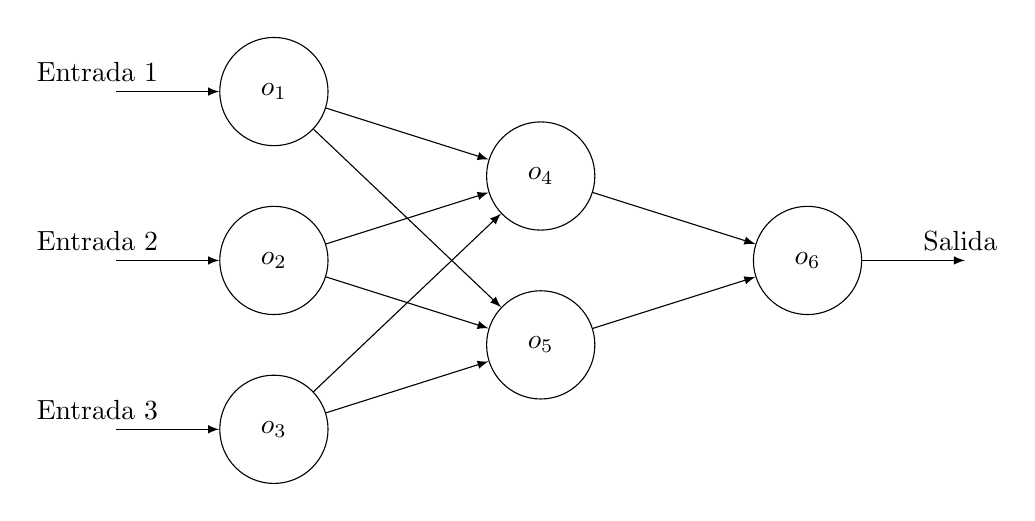
\begin{tikzpicture}[
plain/.style={
  draw=none,
  fill=none,
  },
net/.style={
  matrix of nodes,
  nodes={
    draw,
    circle,
    inner sep=10pt
    },
  nodes in empty cells,
  column sep=2cm,
  row sep=-9pt
  },
>=latex
]
\matrix[net] (mat)
{
 $o_1$ & |[plain]| \\
|[plain]| & $o_4$ \\
$o_2$ & |[plain]| & $o_6$ \\
|[plain]| & $o_5$ \\
 $o_3$ & |[plain]| \\ 
};
\foreach \ai [count=\mi ]in {1,3,5}
  \draw[<-] (mat-\ai-1) -- node[above left] {Entrada \mi} +(-2cm,0);
\foreach \ai in {1,3,5}
{\foreach \aii in {2,4}
  \draw[->] (mat-\ai-1) -- (mat-\aii-2);
}
\foreach \ai in {2,4}
  \draw[->] (mat-\ai-2) -- (mat-3-3);
\draw[->] (mat-3-3) -- node[above right] {Salida} +(2cm,0);

\end{tikzpicture}


\end{document}